\chapter{Design of the proposed solution}
\label{ch:DesignOfTheProposedSolution}
\lettrine[lraise=-0.1, lines=2, loversize=0.2]{L}{o}rem itsum
% El planificador desarrollado en esta tésis se compone a su vez de dos módulos bien diferenciados, el primero es el planificador de tareas propiamente dicho, encargado de la planificación de la misión y de su replanificación cuando fuera necesario, el segundo se encuentra a bordo de cada UAV y gestiona el comportamiento de cada equipo, ejecutando el plan que le ha asignado el primer módulo y reaccionando ante cualquier imprevisto de forma segura.

%%% Capi: En los capítulos 3 y 4 puedes coger texto del documento que tenemos hecho con Giuseppe, y del proyecto tuyo de tesis. 

% Se utilizará una aproximación jerárquica, con un planificador de alto nivel encargado de activar distintos controladores de bajo nivel. El planificador de alto nivel detectará las tareas requeridas por los operarios, y las distribuirá de manera centralizada entre los UAVs, planificando las recargas necesarias. Además, este planificador reaccionará en tiempo real ante posibles fallos reasignando tareas y ejecutando planes de contingencia. También tendrá capacidades cognitivas para interaccionar con humanos de manera eficiente. Los planificadores de bajo nivel se encargarán de controlar el movimiento de los UAVs para ejecutar las distintas tareas, por ejemplo volar hacia un lugar a inspeccionar o a la posición de un operario esperando una herramienta. La investigación de la tesis estará centrada en la planificación de alto nivel, y se utilizarán algoritmos del estado del arte para los controladores de bajo nivel.

% Del WP7_Scenarios: Modificar parámetros de una tarea
Once a task has been delivered to the High-Level Planner, in order to change any of its parameters, the Gesture Recognition node should send again the task, keeping the same Task ID and updating only the corresponding parameters. Thus, the High-Level Planner would overwrite it and allocate it again with the new parameters. In the following, a brief description on how to carry out each of the available tasks in the system. It is assumed that there are Low-Level Controllers running on the \glspl{ACW} to perform basic navigation actions, formation control for human worker monitoring, inspection operations, and physical interaction with the human worker (e.g., to pick or deliver a tool). These Low-Level Controllers operate in a known environment, represented by a map (i.e., an occupancy grid map) that also includes the position of obstacles and the power tower.


\section{Node diagram}
\label{sec:NodeDiagram}
%%% Explicar las comunicaciones que hay entre el planner y el manager
%%% Explicar que se ha hecho de forma que toda la inteligencia y las decisiones estén y se tomen en el planner

%% Del WP7_Scenarios: diagrama de nodos y explicacion de los nodos y la informacion intercambiada
Figure \ref{fig:WP7scheme} shows the software architecture in WP7 from a task planning perspective, including the modules involved and their interfaces. High-level decision-making is carried out by two modules: the \textit{High-Level Planner} and the \textit{Agent Behavior Manager}. 

\begin{figure}[ht]
    \hspace{-1cm}
	\scalebox{0.7}{
		\begin{tikzpicture}
    		% WP7 block
    		\node (WP7-Box) at (8.35,0) [fill=gray!3,rounded corners, draw=black!70, densely dotted, minimum height=5cm, minimum width=19.5cm]{}; 
    		
    		% Gesture Recognition
    		\node (GestureRecognition) at (0,0) [text centered, fill=white, draw, rectangle, minimum width=1.5cm, text width=5.5em]{Gesture\\Recognition};
    		
    		\draw[-latex] ($(GestureRecognition) - (1.8,0)$) -- (GestureRecognition);
    		
    		% High-Level Planner
    		\node (HighLevelPlannerBox) at ($(GestureRecognition) + (3.5,0.25)$) [fill=yellow!15,rounded corners, draw=black!70, densely dotted, minimum height=2cm, minimum width=2.5cm]{}; 
    		\node (HighLevelPlanner) at ($(HighLevelPlannerBox) + (0,-0.25)$) [text centered, fill=white, draw, rectangle, minimum width=1.5cm, text width=5.5em]{High-Level\\Planner};
    		\node (Centralized) at ($(HighLevelPlanner) + (0,0.75)$) [text centered]{\small Centralized};
    		
    		\draw[-latex] (GestureRecognition.east) -- node[above]{Task} (HighLevelPlanner);
    		
    		%%%%%%%%%%%%%%%%%%%
    		% UAV 1
    		\node (UAV1) at ($(HighLevelPlanner) + (6.75,1.25)$) [fill=yellow!15,rounded corners, draw=black!70, densely dotted, minimum height=1.7cm, minimum width=5cm]{}; 
    		\node (AgentBehaviourManager1) at ($(UAV1) + (0,-0.25)$) [fill=white, draw, rectangle, text centered, text width=12em]{Agent Behaviour Manager};
    		\node (UAV1-Text) at ($(AgentBehaviourManager1) + (0,0.75)$) [text centered]{\small On board ACW-$1$};	

    		\draw[fill=black] ($ (HighLevelPlanner.east) + (1.715,0) $) arc(-180:180:0.05);
    		\draw[-latex] (HighLevelPlanner.east) -- ($ (HighLevelPlanner.east) + (1.75,0) $) -- ($ (HighLevelPlanner.east) + (1.75,1) $) -- node[above]{Task} node[below]{List} (AgentBehaviourManager1.west);
    		\draw[-latex] ($ (HighLevelPlanner.east) + (1.75,0) $) -- node[above]{Feedback} (HighLevelPlanner.east);
    		
    		%%%%%%%%%%%%%%%%%%%
    		
    		% Dots
    		\node (Dots2) at ($(UAV1) + (0,-1.25)$) [text centered]{\dots};
    		
    		%%%%%%%%%%%%%%%%%%%
    		
    		% UAV N
    		\node (UAVN) at ($(HighLevelPlanner) + (6.75,-1.25)$) [fill=yellow!15,rounded corners, draw=black!70, densely dotted, minimum height=1.7cm, minimum width=5cm]{}; 
    		\node (AgentBehaviourManagerN) at ($(UAVN) + (0,-0.25)$) [fill=white, draw, rectangle, text centered, text width=12em]{Agent Behaviour Manager};
    		\node (UAVN-Text) at ($(AgentBehaviourManagerN) + (0,0.75)$) [text centered]{\small On board ACW-$N$};	

    		\draw[-latex] (HighLevelPlanner.east) -- ($ (HighLevelPlanner.east) + (1.75,0) $) -- ($ (HighLevelPlanner.east) + (1.75,-1.5) $) -- node[above]{Task} node[below]{List} (AgentBehaviourManagerN.west);
    		
    		%%%%%%%%%%%%%%%%%%%
    		
    		% Lower-Level Controllers
    		\node (LowerLevelControllers) at ($(HighLevelPlanner) + (13.25,0)$) [text centered, fill=white, draw, rectangle, minimum width=1.5cm, text width=5.5em]{Lower-Level\\Controllers};
    		
    		\draw[-latex] (LowerLevelControllers.east) -- ($(LowerLevelControllers) + (1.8,0)$);
    		
    		\draw[fill=black] ($ (LowerLevelControllers.west) + (-1.535,0) $) arc(-180:180:0.05);
    		\draw[-latex] (AgentBehaviourManager1.east) -- ($ (LowerLevelControllers.west) + (-1.5,1) $) -- ($ (LowerLevelControllers.west) + (-1.5,0) $) --  node[above]{Task}
    	    node[below]{Params}	(LowerLevelControllers.west);
    		\draw[-latex] (LowerLevelControllers.west) -- ($ (LowerLevelControllers.west) + (-1.5,0) $) -- ($ (LowerLevelControllers.west) + (-1.5,1) $) -- node[above]{Task}
    	    node[below]{Result}	(AgentBehaviourManager1.east);
    		\draw[-latex] (AgentBehaviourManagerN.east) -- ($ (LowerLevelControllers.west) + (-1.5,-1.5) $) -- ($ (LowerLevelControllers.west) + (-1.5,0) $) -- (LowerLevelControllers.west);
    		\draw[-latex] (LowerLevelControllers.west) -- ($ (LowerLevelControllers.west) + (-1.5,0) $) -- ($ (LowerLevelControllers.west) + (-1.5,-1.5) $) -- 
    		node[above]{Task}
    		node[below]{Result} (AgentBehaviourManagerN.east);
    		
    		%%%%%%%%%%%%%%%%%%%%%
    		
    		\node (RealUAVs) at ($(WP7-Box.south) + (2,-1.25)$) [text centered, fill=white, draw, rectangle, minimum width=1.5cm, text width=6em]{ACWs\\autopilot};
    		\node (Humans) at ($(WP7-Box.south) + (-2,-1.25)$) [text centered, fill=white, draw, rectangle, minimum width=1.5cm, text width=6em]{Humans\\Tracker};
    		
    		\draw[-latex] (RealUAVs.north) -- node[right]{Pose, Battery, State} ($(WP7-Box.south) + (2,0)$);
    		\draw[-latex] ($(WP7-Box.south) + (2,0)$) -- (RealUAVs.north);
    		\draw[-latex] (Humans.north) -- node[left]{Pose} ($(WP7-Box.south) + (-2,0)$);
		
	    \end{tikzpicture}}
	\caption{WP7 Software architecture: Modules and interfaces.}
	\label{fig:WP7scheme}
\end{figure}

The \textit{High-level Planner} is the centralized module of the software architecture and runs on a ground station. This module is in charge of task planning, i.e., it decides which tasks will be assigned to each \gls{ACW}. The system knows the available \glspl{ACW} thanks to the feedback provided by the Terabee~ \gls{RTPS}. At this stage, battery constraints and \gls{ACW} positions and capabilities are taken into consideration. Such information is supplied at a constant rate (to be defined). The number and type of available \glspl{ACW} can be specified before the mission starts via a configuration file. 

The \textit{Agent Behavior Manager} is a distributed module running on board each \gls{ACW}. This module mainly runs a state machine implemented as a \gls{BT} which governs the \gls{ACW} to perform each of the assigned tasks. Each \gls{BT} monitors the \gls{ACW}'s battery and task status and reacts to any possible failure or unexpected event, requesting a new re-planning to the High-Level Planner in case of need. In addition, the \textit{ACW autopilot} and \textit{Human Tracker} nodes supply for the ACW state and human worker pose, respectively. This information is used for monitoring and tool delivery tasks.  

The data interfaces for each module in the software architecture are listed in Table~\ref{tab:interfaces}, while the data explanation is provided in Table~\ref{tab:shareddata}.

\begin{table}[ht]
    \centering
    \caption{Description of the data interfaces for each software module.}
    \label{tab:interfaces}
    \small
    \begin{tabular}{|p{0.25\columnwidth}|p{0.25\columnwidth}|p{0.4\columnwidth}|}
      \hline
      \multicolumn{1}{|c}{\textbf{Module Name}} & \multicolumn{1}{|c|}{\textbf{Input Data}} & \multicolumn{1}{c|}{\textbf{Output Data}}\\ \hline \hline
      Gesture Recognition & Images & \textbf{Task, defined by:} Task ID, Task Type, Monitoring Distance, Monitoring Number, WP List, Tool ID (some task parameters will be ignored depending on Task Type) \\ \hline
      
      High-Level Planner & Task, Feedback (Agent Beacon, BatteryEnough, \gls{BT} info), Humans' Pose, \glspl{ACW}' Pose, Battery and State & Task List adding to each one its extra parameters result of the planning (Formation and/or List of \glspl{ACW}' IDs) \\\hline
      
      Agent Behaviour Manager & Task List, Result (Low-Level Result), Human Pose, \glspl{ACW} Pose, Battery and State & Params needed by Low-Level Controllers (depending on Task Type) \\ \hline
      
      Low-Level Controllers & Params (depending on Task Type) & Result \\ \hline
      
      Humans Tracker &  & Pose \\ \hline
      
      \gls{ACW} autopilot & Low-Level orders & Pose, Battery and State \\ \hline
      
    \end{tabular}
\end{table}
  
\begin{table}[htb]
    \centering
    \caption{Description of data types.}
    \label{tab:shareddata}
    \small
    \begin{tabular}{|p{0.2\columnwidth}|p{0.15\columnwidth}|p{0.55\columnwidth}|}
      \hline
      \multicolumn{1}{|c}{\textbf{Data name}} & \multicolumn{1}{|c|}{\textbf{Data type}} & \multicolumn{1}{c|}{\textbf{Comment}} \\ \hline \hline
      
      Task ID & String & Unique identifier of each task \\ \hline
      
      Task Type & Integer & Task type indicator: m/M, i/I or d/D \\ \hline
      
      Human Target ID & String & Unique identifier of each human worker. The position of the human target and other needed info is supposed to be known and accessible via its ID. \\ \hline
      
      Monitoring Distance & Float & Distance from which the \gls{ACW} surveil the worker during a safety monitoring task \\ \hline
      
      Monitoring Number & Integer & Number of \glspl{ACW} that are required in formation for a certain safety monitoring task \\ \hline
      
      WP List & List of $3$ float tuples ($x$, $y$, and $z$) & List of waypoints to be inspected \\ \hline
      
      List of \glspl{ACW}' IDs & List of Strings & List of the unique identifiers of the \glspl{ACW} that have been selected for a task that requires multiple \glspl{ACW} \\ \hline
      
      Formation & Integer & Indicates which of the predefined types of formations should be used for monitoring (e.g., circle, triangle) \\ \hline
      
      Tool ID & String & Unique identifier of the tool to be delivered \\ \hline
      
      \gls{ACW} Pose & geometry\_msgs /PoseStamped & \gls{ACW} Position and orientation \\ \hline
      
      \gls{ACW} Battery & sensors\_msgs /BatteryState & Percentage of battery in the \gls{ACW}\\ \hline
      
      Battery Enough & Boolean & Result of computing if an \gls{ACW} will have enough battery for its current task \\ \hline
      
      Agent Beacon & String, Integer & \gls{ACW} unique ID and integer defining the type of \gls{ACW} (Safety, Inspect, or Physical Interaction). Used as heartbeat to detect new \glspl{ACW} \\ \hline
      
      \gls{BT} info & String list & Status of each \gls{BT} node: which are Running, which are IDLE, which just returned SUCCESS, and which just returned FAILURE \\ \hline
      
      Lower-Level Result & Boolean & Result of the Low-Level Controllers after a call \\ \hline
      
    \end{tabular}
\end{table}

\section{Centralized module: task planner}
\label{sec:Centralized module:TaskPlanner}
%% Protocolo de desconexión
%% Protocolo de pérdida de batería
%% Que ocurre cuando una tarea termina
%% Replanificaciones de tareas: restricciones a la hora de planificar o replanificar

\section{Distributed module: behavior manager}
\label{sec:Distributed module: behavior manager}
%%% Explicar que se ha hecho con árboles de comportamiento en paralelo a algunos procesos de ros

%% Máquinas de estados vs árboles de comportamiento
% Una vez asimilado el contexto y los requisitos del proyecto, y antes de proceder con el diseño de la solución, se dedicó un tiempo a estudiar las diferencias entre las máquinas de estados finitas (FSM), con las cuales se estaba familiarizado en aquel momento, y los árboles de comportamiento (BT), de los cuales se desconocía completamente su existencia y funcionamiento. Durante este tiempo no solo se prestó atención a las ventajas e inconvenientes de cada herramienta, sino que también se estudiaron las diferentes librerías para C++, preferiblemente compatibles con ROS, que estaban disponibles [1][2][3][4] y se valoró la calidad de la documentación, la cantidad de ejemplos, cruciales para aprender rápidamente a usar una librería cuando aún se es un usuario poco experimentado del lenguaje de programación, la facilidad de uso y el soporte de la librería entre otras cosas. Aunque la cantidad de personas que emplean librerías de FSM es mayor que en el caso de los BT, y por tanto, es mucho más probable encontrar información en foros de Internet relativa a algún detalle concreto que se necesite y que no esté bien documentado, las ventajas que ofrecen los árboles de comportamiento frente a las máquinas de estado finitas fueron determinantes para decidir emplear este tipo de arquitecturas. Tras una primera formación empleando una librería para BT que ya había sido usada puntualmente por un miembro del grupo [2], se descartó como librería a emplear por la escasa documentación y la falta de características que se consideraban necesarias. Finalmente se encontró una librería que parecía tener una documentación bastante mejor, soporte y mantenimiento aún activos y ejemplos simples de código que se podían emplear como punto de partida [3], y que además venía acompañada de una herramienta para diseñar BT gráficamente [4]. El punto negativoes que no parece tener aún muchos usuarios ni un apartado de preguntas y comentarios, y por tanto, ante cualquier problema o duda con la librería, no se dispondrá de ningún tipo de ayuda.

%% Diseño del árbol de comportamiento
% Diseñar el árbol de comportamiento no fue una labor trivial, ya que se estaba habituado a diseñar pensando en máquinas de estado, pero no pensando en árboles de comportamiento. Además, para cada comportamiento deseado no hay una única implementación posible, lo que hace más complicado el diseño cuando no se tiene la intuición suficiente para saber qué forma es mejor. Para tratar de ganar experiencia con la que desarrollar cierta intuición y los conocimientos necesarios para elaborar desde cero un BT, se dedicó un tiempo a reunir y estudiar toda la información posible sobre los árboles de comportamiento que se encontrara por Internet [5][6][7]. Esto fue posible gracias a que los BT sí que son algo más común en el desarrollo de videojuegos [7]. El diseño del BT no ha permanecido invariante desde que se hizo, sino que ha sufrido modificaciones puntuales fruto de reuniones y revisiones del trabajo. Estas modificaciones principalmente buscaban solucionar algún problema detectado ya fuera en algún re-estudio teórico o tras la observación de algún comportamiento indeseado en pruebas de simulación. Antes mostrar y proceder con la explicación del funcionamiento del diseño de BT propuesto, se comentarán brevemente los tipos de nodos disponibles en la librería seleccionada y el funcionamiento de cada uno de ellos.

% Cambiar por una figura hecha con la librería tikz
\begin{figure}[htbp]
    \centering
    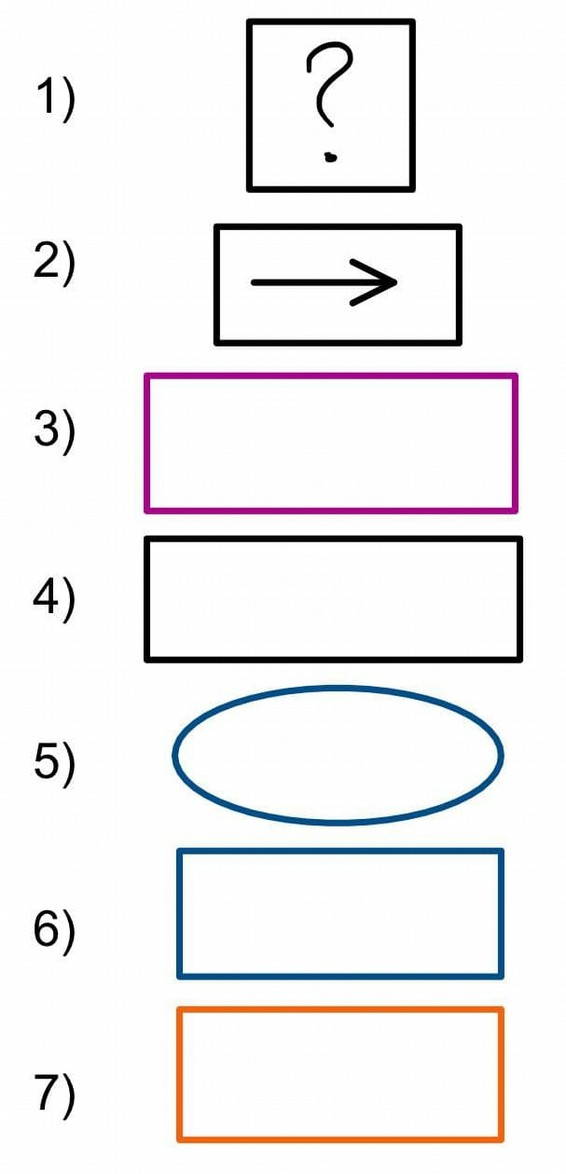
\includegraphics[width=0.4\linewidth]
    {DesignOfTheProposedSolution/figures/BT_node_type.png}
    \caption{Different types of nodes that can be found in a \gls{BT} according to their color and symbol}
    \label{fig:BT_legend}
\end{figure}

%% Del WP7_Scenarios
Behaviour Trees are a more advanced mechanism to implement Finite State Machines, working like them but with improvements in terms of composability, configurability and reusability. Behaviour Trees are made up of control nodes, decorator nodes, and leaf nodes. Control nodes could be either \textit{Fallback} nodes (represented with a question mark), which try success calling one by one each of their children, or \textit{Sequence} nodes (represented with an arrow), which call their children in order if the previous one have returned success. Fallback nodes return success if one of its children does it, failure if none of them return success, and running if a children returns running. On the other hand, Sequence nodes return success when all children have been called in order and have returned success. If any of them returns failure, the sequence is broken and the sequence node returns failure too. When a child returns running, sequence node does it too. A control node could also be \textit{Reactive} (represented in a purple box), which means that its already called children are called again in the next iteration. A child node could be another control node, a decorator node or a leaf node. A decorator node (represented in an orange box) can only have one child (of any type) and its function is programmable (e.g., modifying its child result or retrying calling its child a number of times). Leaf nodes could be condition nodes (represented in an elliptical shaped box) that check a condition and return either success or failure, or action nodes (represented in a rectangular box) that take longer to execute and could also return running).


\subsection{Main tree}
\label{sec:MainTree}
%%% Recalcar que se ha hecho de forma que toda la inteligencia y las decisiones estén y se tomen en el planner
%%% Hablar aqui dentro de como se gestionan las desconexiones, la batería y las replanificaciones
%% Protocolo de desconexión
%% Protocolo de pérdida de batería
%% Que ocurre cuando una tarea termina

% Del WP7_Scenarios
\begin{figure}[ht]
	\begin{center}
		\scalebox{0.9}{
			\begin{tikzpicture}
        		\node (MainTree) at (0,0) [text centered, fill=white, draw, rectangle, minimum width=1.5cm, text width=5.5em]{Main Tree};

        		%%%%%%%%%%%%%%%%%%%%% SECOND LEVEL
        		
        		\node (RootFallback) at ($(MainTree) + (0,-1)$) [text centered, fill=magenta!5, draw=magenta, rectangle, minimum width=0.5cm, text width=0.5em]{\textbf{?}};
        		\draw[-latex] (MainTree.south) -- (RootFallback.north);
        		
        		\node (MissionOverSequence) at ($(RootFallback) + (-3,-1.5)$) [text centered, fill=white, draw, rectangle, minimum width=1.5cm, text width=1.5em]{$\longrightarrow$};
        		\draw[-latex] (RootFallback.south) -- (MissionOverSequence.north);
        	    
        		\node (ForceRunning) at ($(RootFallback) + (3, -1.5)$) [text centered, fill=orange!5, draw=orange, rectangle, minimum width=1.5cm, text width=5.5em]{Force Running};
        		\draw[-latex] (RootFallback.south) -- (ForceRunning.north);
        		
        		\node (MissionFallback) at ($(ForceRunning) + (0,-1.5)$) [text centered, fill=magenta!5, draw=magenta, rectangle, minimum width=0.5cm, text width=0.5em]{\textbf{?}};
        		\draw[-latex] (ForceRunning.south) -- (MissionFallback.north);
        		
        		%%%%%%%%%%%%%%%%%%%%% THIRD LEVEL
        		\node (MissionOver) at ($(MissionOverSequence) + (-1.75,-1.5)$) [text centered, fill=white, draw, ellipse, minimum width=1.5cm, text width=5.5em]{Mission Over?};
        		\draw[-latex] (MissionOverSequence.south) -- (MissionOver.north);
        		\node (BackToStation) at ($(MissionOverSequence) + (1.75, -1.5)$) [text centered, fill=white, draw, rectangle, minimum width=1.5cm, text width=5.5em]{Back To Station};
        		\draw[-latex] (MissionOverSequence.south) -- (BackToStation.north);
        		
        		\node (IdleSequence) at ($(MissionFallback) + (-4.25,-1.25)$) [text centered, fill=magenta!5, draw=magenta, rectangle, minimum width=1.5cm, text width=1.5em]{$\longrightarrow$};
        		\draw[-latex] (MissionFallback.south) -- (IdleSequence.north);
        		\node (WaitFallback) at ($(MissionFallback) + (4.25,-1.25)$) [text centered, fill=magenta!5, draw=magenta, rectangle, minimum width=0.5cm, text width=0.5em]{\textbf{?}};
        		\draw[-latex] (MissionFallback.south) -- (WaitFallback.north);
        		
        		\node (Inverter) at ($(IdleSequence) + (-3, -1.5)$) [text centered, fill=orange!5, draw=orange, rectangle, minimum width=1.5cm, text width=5.5em]{Inverter};
        		\draw[-latex] (IdleSequence.south) -- (Inverter.north);
        		\node (TaskSequence) at ($(IdleSequence) + (2.5,-1.5)$) [text centered, fill=magenta!5, draw=magenta, rectangle, minimum width=1.5cm, text width=1.5em]{$\longrightarrow$};
        		\draw[-latex] (IdleSequence.south) -- (TaskSequence.north);
        		\node (IsBatteryFull) at ($(WaitFallback) + (-1.75,-1.5)$) [text centered, fill=white, draw, ellipse, minimum width=1.5cm, text width=5.5em]{Is Battery Full?};
        		\draw[-latex] (WaitFallback.south) -- (IsBatteryFull.north);
        		\node (Recharge) at ($(WaitFallback) + (1.75, -1.5)$) [text centered, fill=white, draw, rectangle, minimum width=1.5cm, text width=6.5em]{Recharge};
        		\draw[-latex] (WaitFallback.south) -- (Recharge.north);
        		
        		%%%%%%%%%%%%%%%%%%%%% FOURTH LEVEL
        		
        		\node (Idle) at ($(Inverter) + (0,-1.5)$) [text centered, fill=white, draw, ellipse, minimum width=1.5cm, minimum height=1.35cm, text width=5.5em]{Idle?};
        		\draw[-latex] (Inverter.south) -- (Idle.north);
        		\node (IsBatteryEnough) at ($(TaskSequence) + (-1.75,-1.5)$) [text centered, fill=white, draw, ellipse, minimum width=1.5cm, text width=5.5em]{Is Battery Enough?};
        		\draw[-latex] (TaskSequence.south) -- (IsBatteryEnough.north);
        		\node (PerformTaskTree) at ($(TaskSequence) + (1.75, -1.5)$) [text centered, fill=white, draw, rectangle, minimum width=1.5cm, text width=6.5em]{Perform Task Tree};
        		\draw[-latex] (TaskSequence.south) -- (PerformTaskTree.north);
        		
        		%\draw[-latex] (.south) -- (.north);
		    \end{tikzpicture}}
		\caption{Behavior Tree: Main tree}
		\label{fig:MainTree}
	\end{center}
	\vspace{-1em}
\end{figure}

Each Agent Behavior Manager implements several interconnected \gls{BT}. The \emph{Main tree} is depicted in Fig.~\ref{fig:MainTree}. This \gls{BT} checks whether the mission is over (a mission would represent the working session, not a single task, i.e., whether the \gls{ACW} is ready to be turned off) and otherwise, whether the \gls{ACW} has any task to perform. If so, the battery level is checked and, depending on the result, either the corresponding task is executed (sub-tree represented in Fig.~\ref{fig:TasksTree}) or the \gls{ACW} is guided to a recharging station\footnote{Both Safety, Inspection and Physical-ACW provide an input interface to guide the \gls{ACW} to the charging station. In other words, among the low-level controller capabilities, there is a "reach this point". The location of the charging stations is known in advance or provided as input by the High-Level Planner/Behavior Tree.}. The \gls{BT} is also prepared to be safe against a loss of connection with the centralized module. Both unexpected events are managed flushing the task queue for the \gls{ACW} to recharging, while giving the High-Level Planner control to decide when it is the best time to stop recharging (the High-Level Planner just needs to assign tasks again so that the \gls{ACW} start working back).

\begin{figure}[ht]
	\begin{center}
		\scalebox{0.6}{
			\begin{tikzpicture}
			    \node (PerformTaskTree) at (0,0) [text centered, fill=white, draw, rectangle, minimum width=1.5cm, text width=5.5em]{Perform Task Tree};
        		
        		\node (TaskFallback) at ($(PerformTaskTree) + (0,-1.5)$) [text centered, fill=magenta!5, draw=magenta, rectangle, minimum width=0.5cm, text width=1.5em]{\textbf{?}};
        		\draw[-latex] (PerformTaskTree.south) -- (TaskFallback.north);
        		
        		\node (MonitorSequence) at ($(TaskFallback) + (-6.5,-1.5)$) [text centered, fill=magenta!5, draw=magenta, rectangle, minimum width=1.5cm, text width=1.5em]{$\longrightarrow$};
        		\draw[-latex] (TaskFallback.south) -- (MonitorSequence.north);
        		\node (InspectSequence) at ($(TaskFallback) + (0,-1.5)$) [text centered, fill=magenta!5, draw=magenta, rectangle, minimum width=1.5cm, text width=1.5em]{$\longrightarrow$};
        		\draw[-latex] (TaskFallback.south) -- (InspectSequence.north);
        		\node (DeliverSequence) at ($(TaskFallback) + (6.5,-1.5)$) [text centered, fill=magenta!5, draw=magenta, rectangle, minimum width=1.5cm, text width=1.5em]{$\longrightarrow$};
        		\draw[-latex] (TaskFallback.south) -- (DeliverSequence.north);
        		
        		\node (IsTaskMonitor) at ($(MonitorSequence) + (-1.5,-2)$) [text centered, fill=white, draw, ellipse, minimum width=1.5cm, text width=5.5em]{Is Task Safety?};
        		\draw[-latex] (MonitorSequence.south) -- (IsTaskMonitor.north);
        		\node (MonitorTree) at ($(MonitorSequence) + (1.5, -2)$) [text centered, fill=white, draw, rectangle, minimum width=1.5cm, text width=6.5em]{Safety Task Tree};
        		\draw[-latex] (MonitorSequence.south) -- (MonitorTree.north);
        		\node (IsTaskInspect) at ($(InspectSequence) + (-1.5,-2)$) [text centered, fill=white, draw, ellipse, minimum width=1.5cm, text width=5.5em]{Is Task Inspect?};
        		\draw[-latex] (InspectSequence.south) -- (IsTaskInspect.north);
        		\node (InspectTree) at ($(InspectSequence) + (1.5, -2)$) [text centered, fill=white, draw, rectangle, minimum width=1.5cm, text width=6.5em]{Inspect Task Tree};
        		\draw[-latex] (InspectSequence.south) -- (InspectTree.north);
        		\node (IsTaskDeliver) at ($(DeliverSequence) + (-1.5,-2)$) [text centered, fill=white, draw, ellipse, minimum width=1.5cm, text width=5.5em]{Is Task Physical?};
        		\draw[-latex] (DeliverSequence.south) -- (IsTaskDeliver.north);
        		\node (DeliverTree) at ($(DeliverSequence) + (1.5, -2)$) [text centered, fill=white, draw, rectangle, minimum width=1.5cm, text width=6.5em]{Physical Task Tree};
        		\draw[-latex] (DeliverSequence.south) -- (DeliverTree.north);
        		
		    \end{tikzpicture}}
		\caption{Behavior Tree: Perform Task Tree.}
		\label{fig:TasksTree}
	\end{center}
\end{figure}

Figures~\ref{fig:MonitorTree},~\ref{fig:InspectTree} and~\ref{fig:DeliverToolTree} represent the sub-trees that run Safety, Inspection, and Physical tasks, respectively. They all guide the \gls{ACW} close to where the tasks needs to be performed (e.g., close to a worker to monitor or a place to inspect) and then, the corresponding Lower-Level Controller is called. These Lower-Level Controllers run on board the corresponding \gls{ACW}s and must communicate their results (success or failure) asynchronously back to the Agent Behavior Manager, so that the Behaviour Tree could continue running.


% Information exchanges 
% Information interfaces/channels
% Takeovers
\subsection{Inspection task tree}
\label{sec:InspectionTaskTree}
% Del WP7_Scenarios
\textbf{High-Level Planner inputs}: Task ID, Task Type and Waypoint List (the rest will be ignored).

\textbf{Description}: the High-Level Planner, from the list of waypoints, will decide how many \glspl{ACW} are required and which part of the waypoint list is assigned to each one. Then, it would send to each corresponding Agent Behavior Manager the task parameters, including a list with the IDs of the selected~ glspl{ACW}. The same information is forwarded to the Lower-Level Controllers when the BT calls them (see Fig.~\ref{fig:InspectTree}). Basically, the list of waypoints to be inspected are covered by the assigned \glspl{ACW}, stopping at each of them to take images.  

\begin{figure}[ht]
	\begin{center}
		\scalebox{0.9}{
			\begin{tikzpicture}
			    \node (InspectTree) at (0,0) [text centered, fill=white, draw, rectangle, minimum width=1.5cm, text width=5.5em]{Inspect Tree};
        		
        		\node (InspectTaskSequence) at ($(InspectTree) + (0,-1.5)$) [text centered, fill=magenta!5, draw=magenta, rectangle, minimum width=1.5cm, text width=1.5em]{$\longrightarrow$};
        		\draw[-latex] (InspectTree.south) -- (InspectTaskSequence.north);
        		
        		\node (NearWPFallback) at ($(InspectTaskSequence) + (-1.5,-1.5)$) [text centered, fill=magenta!5, draw=magenta, rectangle, minimum width=0.5cm, text width=0.5em]{\textbf{?}};
        		\draw[-latex] (InspectTaskSequence.south) -- (NearWPFallback.north);
        		\node (Inspect) at ($(InspectTaskSequence) + (1.5,-1.5)$) [text centered, fill=white, draw, rectangle, minimum width=1.5cm, text width=5.5em]{Inspect};
        		\draw[-latex] (InspectTaskSequence.south) -- (Inspect.north);
        		
        		\node (IsUAVnearWP) at ($(NearWPFallback) + (-1.5,-2)$) [text centered, fill=white, draw, ellipse, minimum width=1.5cm, text width=5.5em]{Is \gls{ACW} near WP?};
        		\draw[-latex] (NearWPFallback.south) -- (IsUAVnearWP.north);
        		\node (GoNearWP) at ($(NearWPFallback) + (1.5, -2)$) [text centered, fill=white, draw, rectangle, minimum width=1.5cm, text width=6.5em]{Go near WP};
        		\draw[-latex] (NearWPFallback.south) -- (GoNearWP.north);
		    \end{tikzpicture}
		}
		\caption{Behavior Tree: sub-tree that controls the inspect tasks.}
		\label{fig:InspectTree}
	\end{center}
\end{figure}

\subsection{Monitoring task tree}
\label{sec:MonitoringTaskTree}
% Del WP7_Scenarios
\textbf{High-Level Planner inputs}: Task ID, Task Type, Human Target ID, Monitoring Distance, and Monitoring Number (the rest will be ignored).

\textbf{Description}: the High-Level Planner will assign this task to as many Safety-ACWs as specified Monitoring Number. The formation will be chosen by the High-Level Planner from a set of fixed formations (to be listed) depending on the number of \gls{ACW}. Each selected \gls{ACW} will know a list with the IDs of the \glspl{ACW} selected for the task and the formation that they must take. As shown in Fig. \ref{fig:MonitorTree}, each Agent Behaviour Manager would individually navigate each \gls{ACW} near the human target and then, it would call the corresponding Lower-Level Controller for formation control. Extra \glspl{ACW} could even be added to the formation at any time, just updating the task parameters sending a new task from Gesture Recognition.

\begin{figure}[ht]
	\begin{center}
		\scalebox{0.9}{
			\begin{tikzpicture}
			    \node (MonitorTree) at (0,0) [text centered, fill=white, draw, rectangle, minimum width=1.5cm, text width=5.5em]{Safety Monitoring Tree};
        		
        		\node (MonitorTaskSequence) at ($(MonitorTree) + (0,-1.5)$) [text centered, fill=magenta!5, draw=magenta, rectangle, minimum width=1.5cm, text width=1.5em]{$\longrightarrow$};
        		\draw[-latex] (MonitorTree.south) -- (MonitorTaskSequence.north);
        		
        		\node (NearHumanFallback) at ($(MonitorTaskSequence) + (-1.5,-1.5)$) [text centered, fill=magenta!5, draw=magenta, rectangle, minimum width=0.5cm, text width=1.5em]{\textbf{?}};
        		\draw[-latex] (MonitorTaskSequence.south) -- (NearHumanFallback.north);
        		\node (MonitorHumanTarget) at ($(MonitorTaskSequence) + (1.5,-1.5)$) [text centered, fill=white, draw, rectangle, minimum width=1.5cm, text width=5.5em]{Safety Monitoring};
        		\draw[-latex] (MonitorTaskSequence.south) -- (MonitorHumanTarget.north);
        		
        		\node (IsUAVnearHumanTarget) at ($(NearHumanFallback) + (-1.5,-2)$) [text centered, fill=white, draw, ellipse, minimum width=1.5cm, text width=5.5em]{Is \gls{ACW} near Human Target?};
        		\draw[-latex] (NearHumanFallback.south) -- (IsUAVnearHumanTarget.north);
        		\node (GoNearHuman) at ($(NearHumanFallback) + (1.5, -2)$) [text centered, fill=white, draw, rectangle, minimum width=1.5cm, text width=6.5em]{Go near Human Target};
        		\draw[-latex] (NearHumanFallback.south) -- (GoNearHuman.north);
		    \end{tikzpicture}
		}
		\caption{Behavior Tree: sub-tree that controls the safety monitoring tasks.}
		\label{fig:MonitorTree}
	\end{center}
	\vspace{-1em}
\end{figure}

\subsection{Tool delivery task tree}
\label{sec:ToolDeliveryTaskTree}
% Del WP7_Scenarios
\textbf{High-Level Planner inputs}: Task ID, Task Type, Human Target ID and Tool ID (the rest will be ignored).

\textbf{Description}: After task allocation, the High-Level Planner will send the information to the corresponding Agent Behavior Manager and from there, the Lower-Level Controllers will be called sequentially as shown in Fig. \ref{fig:DeliverToolTree}. Basically, the \gls{ACW} needs to navigate to the station where the tool is, pick it up, navigate back to where the worker is, and start physical interaction to deliver the tool. 

\begin{figure}[ht]
	\begin{center}
		\scalebox{0.5}{
			\begin{tikzpicture}
			    \node (DeliverTree) at (0,0) [text centered, fill=white, draw, rectangle, minimum width=1.5cm, text width=6.5em]{Tool Delivery Tree};
        		
        		\node (DeliverTaskSequence) at ($(DeliverTree) + (0,-1)$) [text centered, fill=magenta!5, draw=magenta, rectangle, minimum width=1.5cm, text width=1.5em]{$\longrightarrow$};
        		\draw[-latex] (DeliverTree.south) -- (DeliverTaskSequence.north);
        		
        		\node (ToolFallback) at ($(DeliverTaskSequence) + (-6.5,-1.5)$) [text centered, fill=magenta!5, draw=magenta, rectangle, minimum width=0.5cm, text width=0.5em]{\textbf{?}};
        		\draw[-latex] (DeliverTaskSequence.south) -- (ToolFallback.north);
        		\node (HumanFallback) at ($(DeliverTaskSequence) + (0,-1.5)$) [text centered, fill=white, draw, rectangle, minimum width=0.5cm, text width=0.5em]{\textbf{?}};
        		\draw[-latex] (DeliverTaskSequence.south) -- (HumanFallback.north);
        		\node (PermissionFallback) at ($(DeliverTaskSequence) + (6.5,-1.5)$) [text centered, fill=magenta!5, draw=magenta, rectangle, minimum width=0.5cm, text width=0.5em]{\textbf{?}};
        		\draw[-latex] (DeliverTaskSequence.south) -- (PermissionFallback.north);
        		
        		\node (hasACWtheTool) at ($(ToolFallback) + (-1.5,-2)$) [text centered, fill=white, draw, ellipse, minimum width=1.5cm, text width=5.5em]{Has  the Tool?};
        		\draw[-latex] (ToolFallback.south) -- (hasACWtheTool.north);
        		\node (PickToolSequence) at ($(ToolFallback) + (1.5,-2)$) [text centered, fill=magenta!5, draw=magenta, rectangle, minimum width=1.5cm, text width=1.5em]{$\longrightarrow$};
        		\draw[-latex] (ToolFallback.south) -- (PickToolSequence.north);
        		\node (IsUAVnearHuman) at ($(HumanFallback) + (-1.5,-2)$) [text centered, fill=white, draw, ellipse, minimum width=1.5cm, text width=5.5em]{Is  near Human Target?};
        		\draw[-latex] (HumanFallback.south) -- (IsUAVnearHuman.north);
        		\node (GoNearHuman) at ($(HumanFallback) + (1.5, -2)$) [text centered, fill=white, draw, rectangle, minimum width=1.5cm, text width=6.5em]{Go near Human Target};
        		\draw[-latex] (HumanFallback.south) -- (GoNearHuman.north);
        		\node (DeliverSequence) at ($(PermissionFallback) + (-2.25,-2)$) [text centered, fill=white, draw, rectangle, minimum width=1.5cm, text width=1.5em]{$\longrightarrow$};
        		\draw[-latex] (PermissionFallback.south) -- (DeliverSequence.north);
        		\node (ForceFailure) at ($(PermissionFallback) + (2.25, -2)$) [text centered, fill=orange!5, draw=orange, rectangle, minimum width=1.5cm, text width=5.5em]{Force Failure};
        		\draw[-latex] (PermissionFallback.south) -- (ForceFailure.north);
        		
        		\node (StationFallback) at ($(PickToolSequence) + (-1.5,-2)$) [text centered, fill=white, draw, rectangle, minimum width=0.5cm, text width=0.5em]{\textbf{?}};
        		\draw[-latex] (PickToolSequence.south) -- (StationFallback.north);
        		\node (PickTool) at ($(PickToolSequence) + (1.5, -2)$) [text centered, fill=white, draw, rectangle, minimum width=1.5cm, text width=6.5em]{Pick Tool};
        		\draw[-latex] (PickToolSequence.south) -- (PickTool.north);
        		\node (hasUAVpermission) at ($(DeliverSequence) + (-3,-2)$) [text centered, fill=white, draw, ellipse, minimum width=1.5cm, text width=5.5em]{Has  permission?};
        		\draw[-latex] (DeliverSequence.south) -- (hasUAVpermission.north);
        		\node (DeliverTool) at ($(DeliverSequence) + (0, -2)$) [text centered, fill=white, draw, rectangle, minimum width=1.5cm, text width=6.5em]{Tool Delivery};
        		\draw[-latex] (DeliverSequence.south) -- (DeliverTool.north);
        		\node (Retreat) at ($(DeliverSequence) + (3, -2)$) [text centered, fill=white, draw, rectangle, minimum width=1.5cm, text width=4.5em]{Retreat};
        		\draw[-latex] (DeliverSequence.south) -- (Retreat.north);
        		\node (WaitFallback) at ($(ForceFailure) + (0,-2)$) [text centered, fill=magenta!5, draw=magenta, rectangle, minimum width=0.5cm, text width=0.5em]{\textbf{?}};
        		\draw[-latex] (ForceFailure.south) -- (WaitFallback.north);
        		
        		\node (IsUAVnearStation) at ($(StationFallback) + (-1.5,-2)$) [text centered, fill=white, draw, ellipse, minimum width=1.5cm, text width=5.5em]{Is \gls{ACW} near Station?};
        		\draw[-latex] (StationFallback.south) -- (IsUAVnearStation.north);
        		\node (GoNearStation) at ($(StationFallback) + (1.5, -2)$) [text centered, fill=white, draw, rectangle, minimum width=1.5cm, text width=6.5em]{Go near Station};
        		\draw[-latex] (StationFallback.south) -- (GoNearStation.north);
        		\node (TimeoutSequence) at ($(WaitFallback) + (-1.5,-2)$) [text centered, fill=white, draw, rectangle, minimum width=1.5cm, text width=1.5em]{$\longrightarrow$};
        		\draw[-latex] (WaitFallback.south) -- (TimeoutSequence.north);
        		\node (Wait) at ($(WaitFallback) + (1.5, -2)$) [text centered, fill=white, draw, rectangle, minimum width=1.5cm, text width=6.5em]{Wait for Permission};
        		\draw[-latex] (WaitFallback.south) -- (Wait.north);
        		
        		\node (Timeout) at ($(TimeoutSequence) + (-3,-2)$) [text centered, fill=white, draw, ellipse, minimum width=1.5cm, text width=5.5em]{Timeout?};
        		\draw[-latex] (TimeoutSequence.south) -- (Timeout.north);
        		\node (GoNearStation) at ($(TimeoutSequence) + (0, -2)$) [text centered, fill=white, draw, rectangle, minimum width=1.5cm, text width=6.5em]{Go near Station};
        		\draw[-latex] (TimeoutSequence.south) -- (GoNearStation.north);
        		\node (DropTool) at ($(TimeoutSequence) + (3, -2)$) [text centered, fill=white, draw, rectangle, minimum width=1.5cm, text width=4.5em]{Drop the Tool};
        		\draw[-latex] (TimeoutSequence.south) -- (DropTool.north);
		    \end{tikzpicture}
		}
		\caption{Behavior Tree: sub-tree that controls the tool delivery tasks.}
		\label{fig:OldDeliverToolTree}
	\end{center}
\end{figure}

% Versión nueva pero sin colorear
\begin{figure}[ht]
	\begin{center}
		\scalebox{0.65}{
			\begin{tikzpicture}
			    \node (DeliverTree) at (0,0) [text centered, fill=white, draw, rectangle, minimum width=1.5cm, text width=6.5em]{Tool Delivery Tree};
			    
			    %%%%%%%%%%%%%%%%%%%%% SECOND LEVEL
        		
        		\node (DeliverTaskSequence) at ($(DeliverTree) + (0,-1)$) [text centered, fill=white, draw, rectangle, minimum width=1.5cm, text width=1.5em]{$\longrightarrow$};
        		\draw[-latex] (DeliverTree.south) -- (DeliverTaskSequence.north);
        		
        		\node (ToolFallback) at ($(DeliverTaskSequence) + (-6.5,-1.5)$) [text centered, fill=white, draw, rectangle, minimum width=0.5cm, text width=0.5em]{\textbf{?}};
        		\draw[-latex] (DeliverTaskSequence.south) -- (ToolFallback.north);
        		\node (HumanFallback) at ($(DeliverTaskSequence) + (0,-1.5)$) [text centered, fill=white, draw, rectangle, minimum width=0.5cm, text width=0.5em]{\textbf{?}};
        		\draw[-latex] (DeliverTaskSequence.south) -- (HumanFallback.north);
        		%\node (PermissionFallback) at ($(DeliverTaskSequence) + (6.5,-1.5)$) [text centered, fill=white, draw, rectangle, minimum width=0.5cm, text width=0.5em]{\textbf{?}};
        		%\draw[-latex] (DeliverTaskSequence.south) -- (PermissionFallback.north);
        		\node (DeliverTool) at ($(DeliverTaskSequence) + (6.5,-1.5)$) [text centered, fill=white, draw, rectangle, minimum width=1.5cm, text width=6.5em]{Tool Delivery};
        		\draw[-latex] (DeliverTaskSequence.south) -- (DeliverTool.north);
        		
        		%%%%%%%%%%%%%%%%%%%%% THIRD LEVEL
        		
        		\node (hasACWtheTool) at ($(ToolFallback) + (-1.5,-2)$) [text centered, fill=white, draw, ellipse, minimum width=1.5cm, text width=5.5em]{Has  the Tool?};
        		\draw[-latex] (ToolFallback.south) -- (hasACWtheTool.north);
        		\node (PickToolSequence) at ($(ToolFallback) + (1.5,-2)$) [text centered, fill=white, draw, rectangle, minimum width=1.5cm, text width=1.5em]{$\longrightarrow$};
        		\draw[-latex] (ToolFallback.south) -- (PickToolSequence.north);
        		\node (IsUAVnearHuman) at ($(HumanFallback) + (-1.5,-2)$) [text centered, fill=white, draw, ellipse, minimum width=1.5cm, text width=5.5em]{Is  near Human Target?};
        		\draw[-latex] (HumanFallback.south) -- (IsUAVnearHuman.north);
        		\node (GoNearHuman) at ($(HumanFallback) + (1.5, -2)$) [text centered, fill=white, draw, rectangle, minimum width=1.5cm, text width=6.5em]{Go near Human Target};
        		\draw[-latex] (HumanFallback.south) -- (GoNearHuman.north);
        		%\node (DeliverSequence) at ($(PermissionFallback) + (-2.25,-2)$) [text centered, fill=white, draw, rectangle, minimum width=1.5cm, text width=1.5em]{$\longrightarrow$};
        		%\draw[-latex] (PermissionFallback.south) -- (DeliverSequence.north);
        		%\node (ForceFailure) at ($(PermissionFallback) + (2.25, -2)$) [text centered, fill=white, draw, rectangle, minimum width=1.5cm, text width=5.5em]{Force Failure};
        		%\draw[-latex] (PermissionFallback.south) -- (ForceFailure.north);
        		
        		%%%%%%%%%%%%%%%%%%%%% FOURTH LEVEL LEFT OF THE SCREEN
        		
        		\node (StationFallback) at ($(PickToolSequence) + (-1.5,-2)$) [text centered, fill=white, draw, rectangle, minimum width=0.5cm, text width=0.5em]{\textbf{?}};
        		\draw[-latex] (PickToolSequence.south) -- (StationFallback.north);
        		\node (PickTool) at ($(PickToolSequence) + (1.5, -2)$) [text centered, fill=white, draw, rectangle, minimum width=1.5cm, text width=6.5em]{Pick Tool};
        		\draw[-latex] (PickToolSequence.south) -- (PickTool.north);
        		%\node (hasUAVpermission) at ($(DeliverSequence) + (-3,-2)$) [text centered, fill=white, draw, ellipse, minimum width=1.5cm, text width=5.5em]{Has  permission?};
        		%\draw[-latex] (DeliverSequence.south) -- (hasUAVpermission.north);
        		%\node (DeliverTool) at ($(DeliverSequence) + (0, -2)$) [text centered, fill=white, draw, rectangle, minimum width=1.5cm, text width=6.5em]{Tool Delivery};
        		%\draw[-latex] (DeliverSequence.south) -- (DeliverTool.north);
        		%\node (Retreat) at ($(DeliverSequence) + (3, -2)$) [text centered, fill=white, draw, rectangle, minimum width=1.5cm, text width=4.5em]{Retreat};
        		%\draw[-latex] (DeliverSequence.south) -- (Retreat.north);
        		%\node (WaitFallback) at ($(ForceFailure) + (0,-2)$) [text centered, fill=white, draw, rectangle, minimum width=0.5cm, text width=0.5em]{\textbf{?}};
        		%\draw[-latex] (ForceFailure.south) -- (WaitFallback.north);
        		
        		%%%%%%%%%%%%%%%%%%%%% FOURTH LEVEL CENTER OF THE SCREEN
        		
        		\node (IsUAVnearStation) at ($(StationFallback) + (-1.5,-2)$) [text centered, fill=white, draw, ellipse, minimum width=1.5cm, text width=5.5em]{Is \gls{ACW} near Station?};
        		\draw[-latex] (StationFallback.south) -- (IsUAVnearStation.north);
        		\node (GoNearStation) at ($(StationFallback) + (1.5, -2)$) [text centered, fill=white, draw, rectangle, minimum width=1.5cm, text width=6.5em]{Go near Station};
        		\draw[-latex] (StationFallback.south) -- (GoNearStation.north);
        		%\node (TimeoutSequence) at ($(WaitFallback) + (-1.5,-2)$) [text centered, fill=white, draw, rectangle, minimum width=1.5cm, text width=1.5em]{$\longrightarrow$};
        		%\draw[-latex] (WaitFallback.south) -- (TimeoutSequence.north);
        		%\node (Wait) at ($(WaitFallback) + (1.5, -2)$) [text centered, fill=white, draw, rectangle, minimum width=1.5cm, text width=6.5em]{Wait for Permission};
        		%\draw[-latex] (WaitFallback.south) -- (Wait.north);
        		
        		%%%%%%%%%%%%%%%%%%%%% FOURTH LEVEL RIGHT OF THE SCREEN
        		
        		%\node (Timeout) at ($(TimeoutSequence) + (-3,-2)$) [text centered, fill=white, draw, ellipse, minimum width=1.5cm, text width=5.5em]{Timeout?};
        		%\draw[-latex] (TimeoutSequence.south) -- (Timeout.north);
        		%\node (GoNearStation) at ($(TimeoutSequence) + (0, -2)$) [text centered, fill=white, draw, rectangle, minimum width=1.5cm, text width=6.5em]{Go near Station};
        		%\draw[-latex] (TimeoutSequence.south) -- (GoNearStation.north);
        		%\node (DropTool) at ($(TimeoutSequence) + (3, -2)$) [text centered, fill=white, draw, rectangle, minimum width=1.5cm, text width=4.5em]{Drop the Tool};
        		%\draw[-latex] (TimeoutSequence.south) -- (DropTool.north);
		    \end{tikzpicture}
		}
		\caption{Behavior Tree: sub-tree that controls the tool delivery tasks.}
		\label{fig:DeliverToolTree}
	\end{center}
\end{figure}

\section{Lower and upper level modules faker}
\label{sec:LowerAndUpperLevelModulesFaker}
%%% GoToWP, Recharge, Monitoring, Inspection, ToolDelivery
%%% Battery sensor
